\subsection{Placement of edge data centres \emph{Ericsson}}
\subsubsection{Proposed research}
There are no clear directions as to what degree the coming mobile networks will be virtualized. The degree of virtualization will determine the distribution of compute resources in the network, bounded by properties such as propagation delay, and cell resource provisioning.

The geographic domain in which users move, the location and size of the \xcloud hosting entity defines the bounds in which the service can perform optimally.

We propose a service performance study into the placement of the \xcloud resources. The study will contrast the service delay performance with the placement of the \xcloud resources ranging from the radio bases station to the adjacent core network, where there the \xcloud node caters for multiple base stations.

\begin{figure}
	\centering
	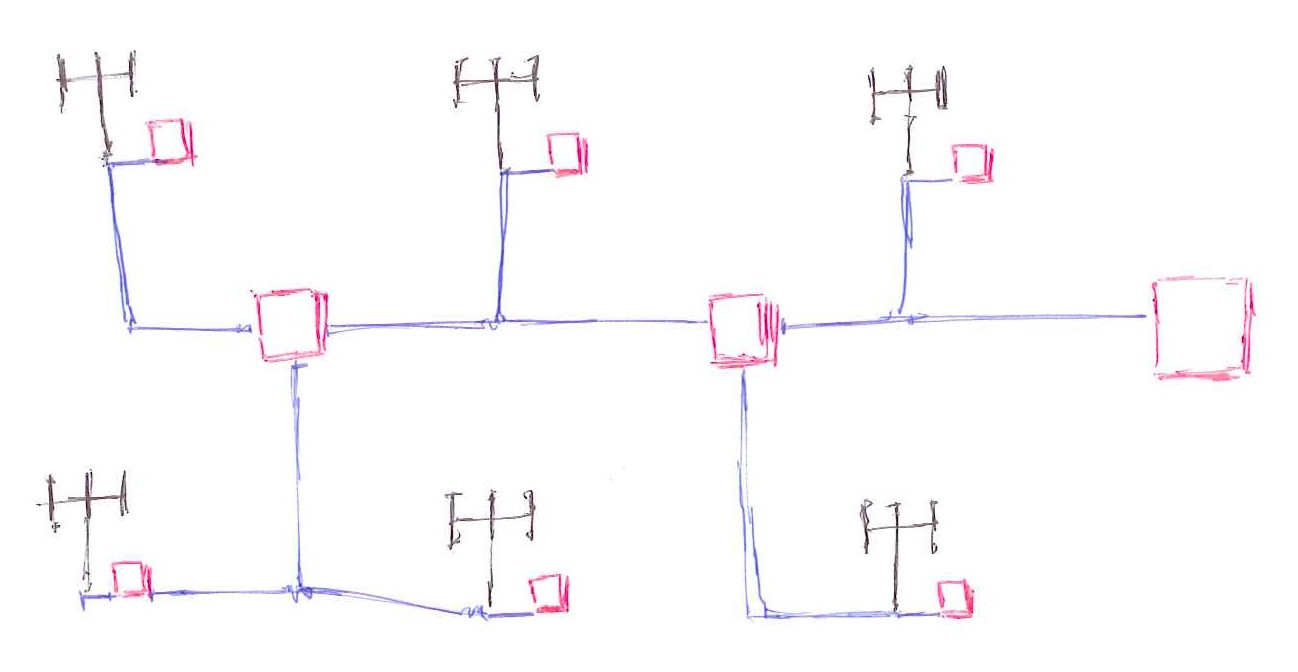
\includegraphics[width=\linewidth]{placement_diagram.jpg}
	\caption{\xcloud placement}
	\label{diagram_placement}
\end{figure}

The service delay will be determined by the additive latency in the mobile network, the level of congestion in the \xcloud node, and the resource shift instigated by user mobility.

We propose to contract the latency experienced by the user with the additional load imposed on the \xcloud infrastructure, as a form of utility.
\subsubsection{Related research}


\subsection{How mobility of user affects network and cloud computing? \emph{Lund}}
\subsubsection{Proposed research}

\subsubsection{Related research}


\subsection{VM placement and migration decisions \emph{Umeå}}
\subsubsection{Proposed research}
In the \xcloud a service will either exists only locally or distributed, but purposely serves a geographically and demographically bounded populous. The units on which the service is hosted are of limited capacity and cannot he universally virtualized as a traditional data center, with relatively unlimited capacity over time. Give the load on each of the nodes and their geographic relevance to the demographic populous they server, services will conceivably need to be mobile, migrating, dispersing, and contracting to minimize such properties as cost, load, and traffic, also taking into account the cost of the migration itself.

We propose research into an appropriate centralized or distributed, load balancing cost function, taking into account :

\begin{itemize}
\item Incurred migration load on host and receiver
\item Incurred migration induced network congestion
\item Network congestion
\item Delay \/ RTT to client to aggregate client base. In other words, minimize delay to aggregate delay/latency to all its served clients. \emph{Perhaps separate research topic preceding this one}
\item Client mobility
\end{itemize}

A property such as energy consumption is perhaps irrelevant to a topology of small data centres as domain of movement is fairly limited and bounded by the demographic service, the rate of which a service migrates is to some extent bounded by the mobility of its users. Nevertheless, energy can become a relevant parameter if the service is allowed to migrate between the \xcloud and a traditional data centre or if the energy profiles of the local \xcloud hosts, is heterogeneous. As the serviced domain is bounds each service by its sociogeographic profile and the fact that latency gains are fairly small accounting for thermal emissions and reuse would be counter productive, and should be dealt with optimally by each node independently. When optimizing for latency, inherent thermal efficiency will conceivably seldom correlate with the service sociogeographic domain. 

\subsubsection{Related research}
Existing research in this area is mainly focuses on load balancing and provisioning between larger distributed data centres with static users.


\subsection{How many devices can be handle by the current infrastructure (latency/bandwidth limits or other requirements) \emph{Umeå} }
\subsubsection{Proposed research}
The number of devices accessing the cloud services is bound to grow significantly with the advent of the internet of things. Most of these devices will communicate over the mobile network. Although the added devices will not necessarily contribute as much data traffic as a user-interaction device, they will significantly add to the congestion to the radio access networks and the adjacent core network. In such a case the, the congestion might result in increased latency in the mobile access network and the adjacent core network.
\subsubsection{Related research}


\subsection{Influence of huge number of (mobile) devices and internet of things \emph{Umeå} }
\subsubsection{Proposed research}
\subsubsection{Related research}


\subsection{Size of edge data centres (number of CPU, memory, etc.) \emph{Ericsson}}
\subsubsection{Proposed research}
\subsubsection{Related research}


\subsection{What type of traffic should be directed to edge data centres? \emph{Lund}}
\subsubsection{Proposed research}
\subsubsection{Related research}


\subsection{Topology of mobile network (antennas detached from BTS) CRAN \emph{Lund}}
\subsubsection{Proposed research}
\subsubsection{Related research}